\section{Introduction}
\label{sec:intro}
Personalized dialogue systems are promising NLP applications for human-computer interaction and emotional companionship. We would expect such systems to have personalities, exhibit emotions, take dialogue acts and even adopt sophisticated strategies \citep{liu2021towards}, which necessitates the research efforts on \textit{Controllable Text Generation}. Despite recent progress in this field \citep{dathathri2019plug,keskar2019ctrl,krause2021gedi}, they mainly tackle single-attribute control, overlooking the fact that human interaction can usually convey multiple attributes simultaneously. Therefore, we explore a novel task of \textit{Multi-Attribute Controllable 
Dialogue Generation}, which can significantly ameliorate the expressiveness, human-likeness, and explainability of chat-bots. However, the numerous combinations of attributes can make the available data for each setting scarce, which poses a great challenge for this task.
% \KZ{We should try not to confuse the words ``attribute'' with aspect. IMO,
% we don't need to introduce the concept of aspect here. Because to the
% model, happy, sad, or man, or women, they are all independent. Normally,
% we say that ``emotion'' is the attribute, and ``happy'' and ``sad'' are its
% values (attribute values). But here since you can have happy and sad being
% 1 at the same time (even though that doesn't really make sense, but i can
% imagine some emotions can co-exists, e.g., sad and angry? So in this case,
% $a_k$ is really just a distinct attribute value. We don't even have to bother
% with the aspect.}
% \ZL{I use the term aspect following previous works. and at least we need a convenient word to refer to (Emotion, Gender, DA). If not aspect, I also need sth. like attribute class, so I will stick to the term.}


% \KZ{Why resort to weighted decoding when the multi-attribute data is scarce? \MY{Agree that there's no logical link between these two. This can be moved to the previous paragraph indicating the complexity and difficulty in multi-aspect generation. In this paragraph, we can focus on saying the normally well-performing weighted decoding in single aspect can exhibit certain challenges when adapted to multi-aspects.}} 
Among previous works, \textit{Weighted Decoding} methods has achieved great success in single-attribute control tasks~\citep{arora2022director,liu-etal-2022-length}. 
Weighted decoding methods learn a token-level attribute classifier, 
which predicts the probability of the text conveying the desired attribute 
given the generation of each token in the vocabulary. 
Then the predicted probabilities are used to 
re-weigh the token generation during decoding to induce the attribute. 
Despite success in single-attribute 
control, they have certain limitations when extended to the multi-attribute case 
by multiplying several attribute predictions from multiple classifiers. Extra 
parameters proportional to the large vocabulary size $|V|$ will be introduced, 
which can grow several times further due to the number of attributes. 
The consequent large number of parameters will not only make the model inefficient, but also harm the generation quality. The model can be prone to overfit since the data for each attribute combination are usually small, which increases the risk of degeneration \citep{holtzman2019curious}. 

To overcome these limitations, we propose \textbf{D}ialog \textbf{A}ttribute \textbf{S}pace \textbf{C}ontroller (\textbf{DASC}). We establish an attribute semantic space where each token in the vocabulary is projected to the space through \textit{Attribute Token Embedding} shared across attributes. The language models' hidden states are also converted to \textit{Attribute Context Embedding} in the space through attribute-specific layers. The attribute space will be trained to make the tokens suitable to convey the desired attribute close to the current context embedding. We can then assign higher weights for the those tokens during decoding.
We will show that DASC can inherit the strong controllability of weighted decoding, 
while also achieving a natural solution of multi-attribute control with the 
interpolation of multiple attribute embeddings in the space. Moreover, 
the shared attribute token embedding also alleviates over-parameterization, 
and improves the robustness of the model.

\begin{figure}[ht]
    \centering
    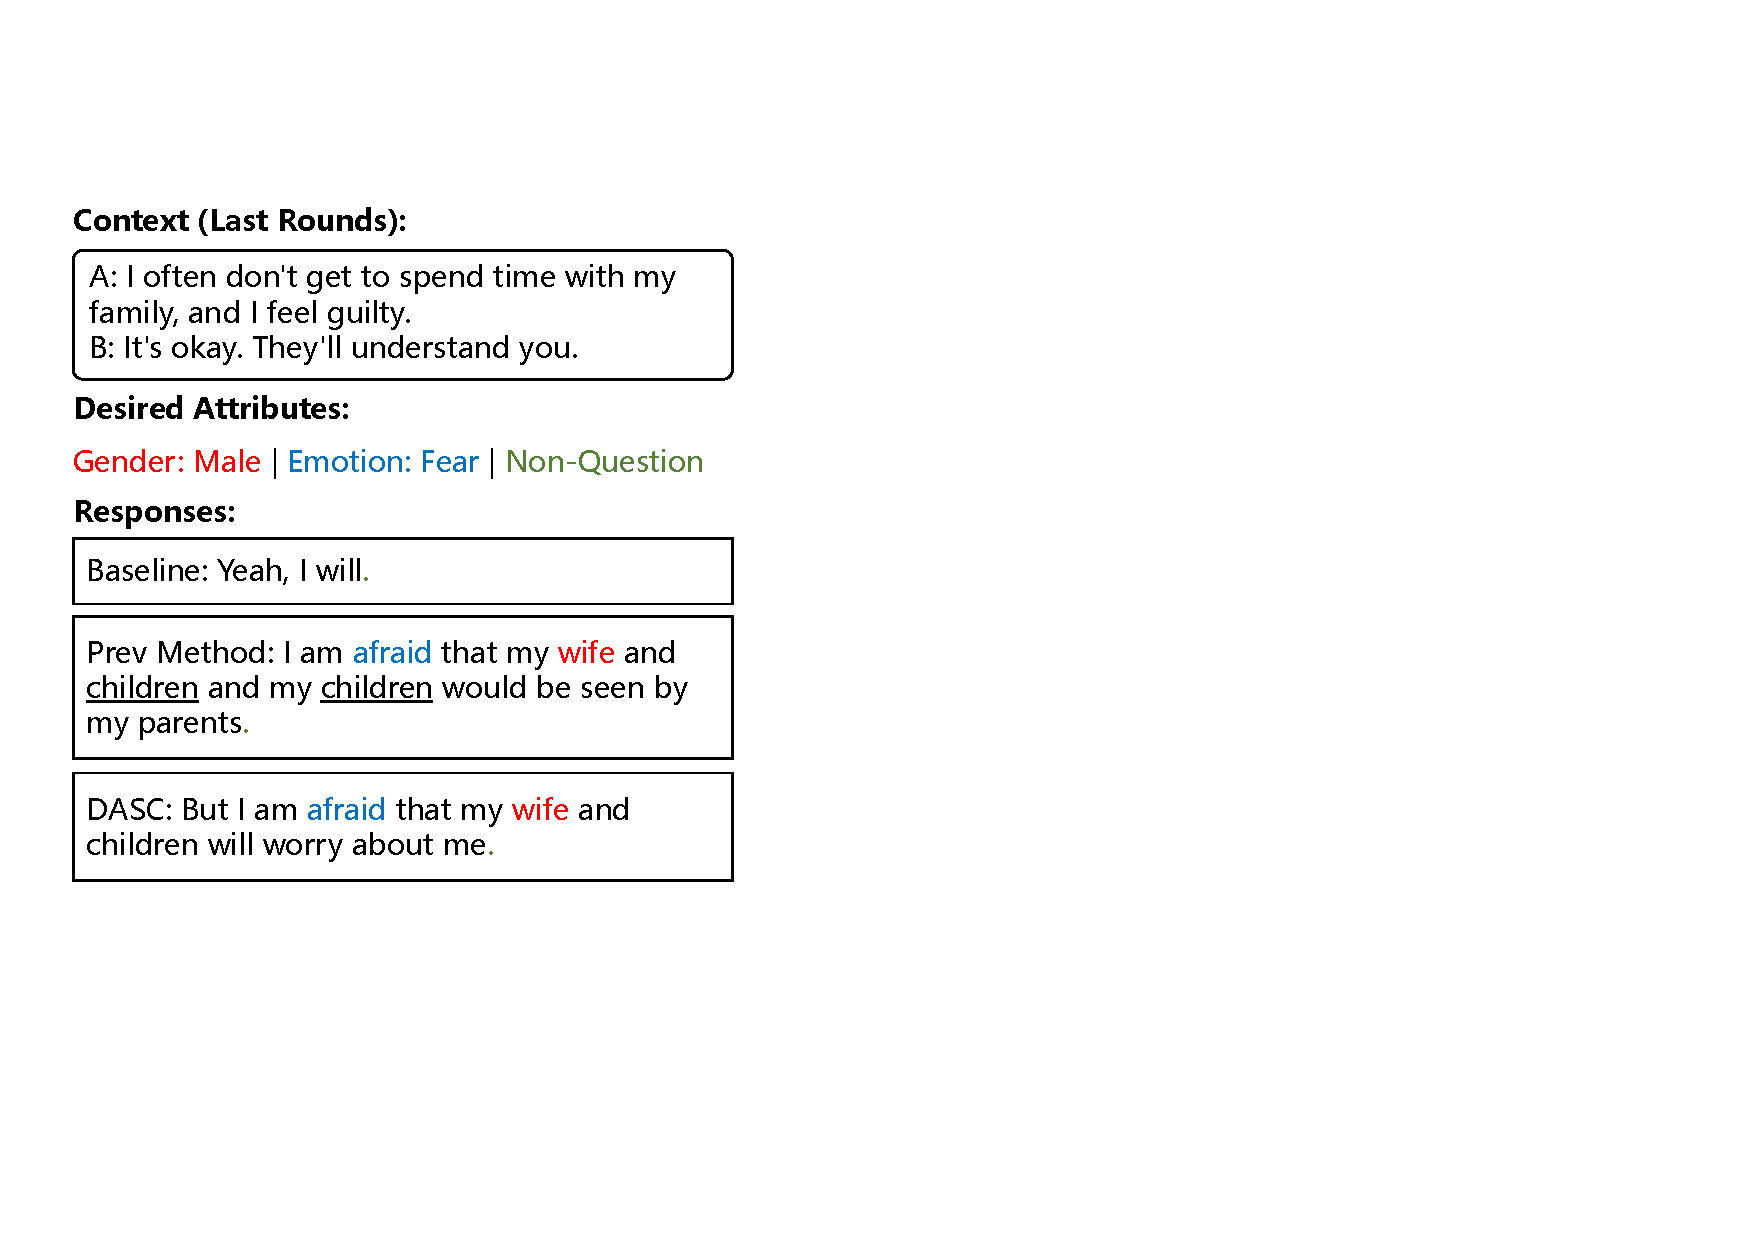
\includegraphics[width=0.75\columnwidth]{figures/teaser_example.pdf}
    \caption{An example of multi-attribute controllable dialogue generation. 
The baseline system doesn't attempt any control and produced a dull response, 
while a previous method of attribute control generated a repetitive and illogical text. DASC successfully gives a response that is both fluent and 
correctly attributed.}
    \label{fig:teaser_example}
\end{figure}

We experiment on an attribute-rich open-domain dialogue dataset \citep{xu2022long} for the simultaneous control of 3 attribute aspects: Gender Style (male, female, neutral), Emotion (8 classes), and a simple division of Dialogue Act 
(question VS non-question). 
As exemplified in \figref{fig:teaser_example}, 
compared to previous methods, DASC achieves strong controllability while 
avoiding low-quality generations in the compositional controlling task. 
Visualization of the attribute token embeddings (in \figref{fig:token_emb}) 
exhibits specific patterns 
that benefit the controlling, compared to the general LM token embeddings. 
We further conducted a robustness test in a out-of-distribution setting and validated that DASC's controllability generalizes.
Our contributions are as follows: 1) We propose semantic space grounded weighted decoding for controllable dialogue generation, which can intuitively solve the multi-attribute control task with the interpolation of embeddings in the space; 2) DASC uses smaller number of parameters than other weighted decoding alternatives while achieving better performance with the design of shared attribute embeddings; 3) DASC can achieve high accuracy on the simultaneous control of 3 aspects while also preserving competitive generation quality in both conventional test settings and out-of-distribution robustness tests.
